\section{Auswertung}
\label{sec:Auswertung}
\subsection{Bestimmung der Halbwertsbreite und Intensität}
DIe Intensitätsverteilung des Röntgenstrahls kann durch eine Gaußfunktion der Form
\begin{equation}
    I(\theta)=\frac{I_0}{\sqrt{2\cdot \pi \cdot \sigma^2}} \cdot \exp\left(-\frac{(\theta-\mu)^2}{2\cdot \sigma^2}\right)+b
\end{equation}
beschrieben werden. Dabei ist $I_0$ die maximale Intensität, $\mu$ der Mittelwert, $\sigma$ die Standardabweichung und $b$ der Untergrund. Die Halbwertsbreite $FWHM$ ist definiert als der Abstand von $\theta$ zu den Punkten, an denen die Intensität auf die Hälfte des Maximums abgefallen ist. Die Halbwertsbreite kann durch die Formel
\begin{equation}
    FWHM = 2\cdot \sqrt{2\cdot \ln(2)}\cdot \sigma
\end{equation}
berechnet werden. Die Daten sind mit Hilfe von Curvefit aus der Python Bibliothek Scipy \cite{scipy} mit einer Gaussfunktion gefittet worden.
Die Messwerte und der Fit sind in Abbildung \ref{fig:Detectorscan} dargestellt. Die Fitparameter betragen
\begin{align*}
    I_0 &= \SI{3.42(0.04)e5}{\per\second}, \\
    \mu &= \SI{0.0031(0.0005)}{\degree}, \\
    \sigma &= \SI{0.0372(0.0004)}{\degree}, \\
    b &= \SI{5.2(0.9)e4}{\per\second}.
\end{align*}
Damit ist die maximale Intensität $I_0=\SI{3.42(0.04)e5}{\per\second}$ und die Halbwertsbreite $FWHM = \SI{0.087(0.001)}{\degree}$.
\begin{figure}[H]
    \centering
    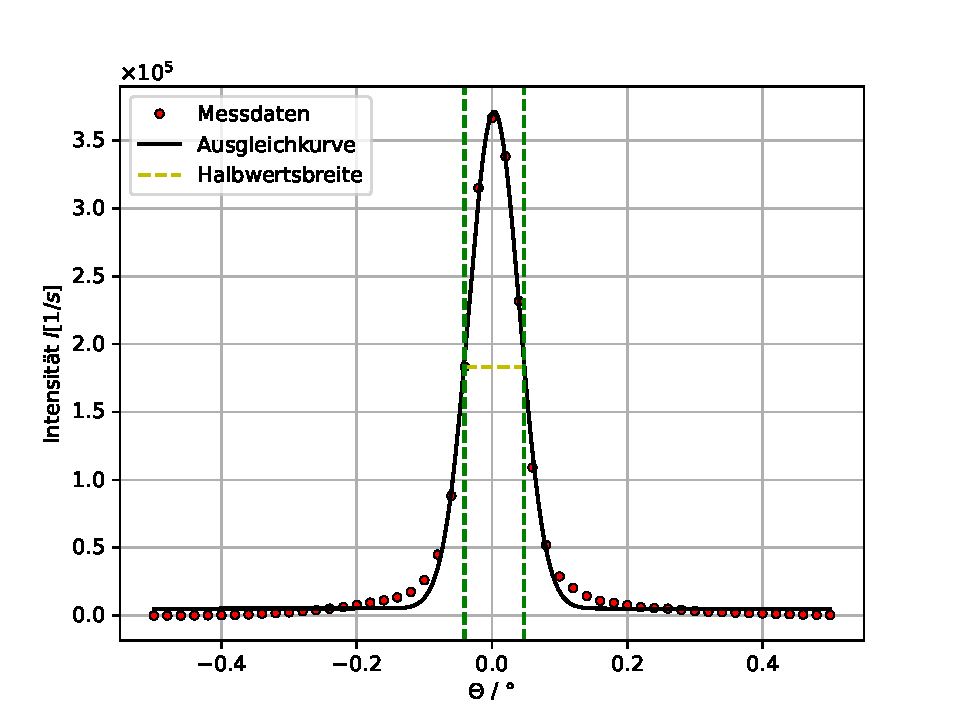
\includegraphics[width=0.8\textwidth]{plots/Detectorscan.pdf}
    \caption{Winkelabhängigkeit der Intensität des Röntgenstrahls}
    \label{fig:Detectorscan}
\end{figure}
\subsection{Bestimmung des Geometriewinkels}
Abbildung \ref{fig:Zscan} zeigt den Z-Scan. Aus der Breite des Intensitätsabfalls, sobald die Probe getroffen wird, 
kann der Strahldurchmesser bestimmt werden. 
Als Grenzen wurden der erste Messpunkt vor dem linearen Abfall und der erste Messpunkt nach dem linearen Abfall gewählt. 
Daraus ergibt sich ein Strahldurchmesser von $d=\SI{0.16}{\milli\meter}$.
\begin{figure}[H]
    \centering
    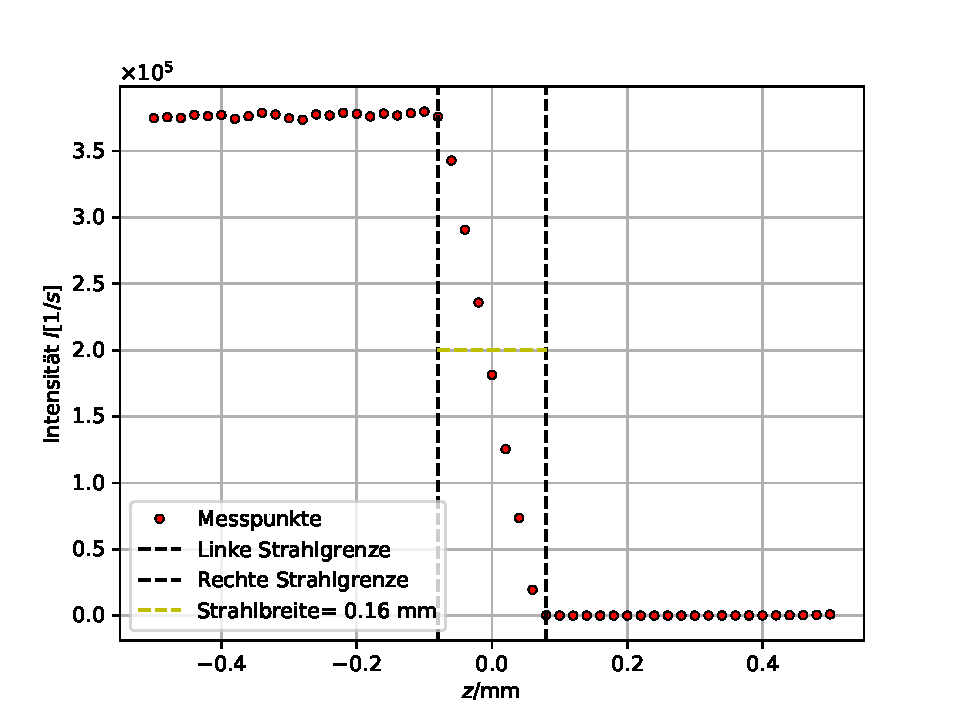
\includegraphics[width=0.8\textwidth]{plots/Zscan.pdf}
    \caption{Z-Scan zur Bestimmung der Strahlbreite}
    \label{fig:Zscan}
\end{figure}
In Abbildung \ref{fig:Xscan} ist der X-Scan dargestellt. An dem Ort an dem sich die Probe befindet fällt die Intensität ab. Daher kann aus der Breite des Abfalls ide Probenbreite 
bestimmt werden. Dafür sind jeweils drei Messpunkte des Randes für eine lineare Ausgleichsgerade $y=a\cdot x+b$ genommen worden. Die Probenbreite wurde bei der halben Intensität gemessen.
Durch Umstellen der Gleichung für die Ausgleichsgerade ergibt sich dann die Position der Ränder. 
Die Parameter der linearen Ausgleichsgerade für die Ränder, welcher mit der Numpy-Funktion Polyfit erstellt worden ist, betragen
\begin{align*}
    a_1 &= \SI{-9e5}{\per\milli\meter\second}, \\
    b_1 &= \SI{-8.5e6}{\milli\meter\second}, \\
    a_2 &= \SI{7.7e5}{\per\milli\meter\second}, \\
    b_2 &= \SI{-5e6}{\milli\meter\second}.
\end{align*}
Damit ergibt sich die Probenbreite zu $d=\SI{22.44}{\milli\meter}$.
\begin{figure}[H]
    \centering
    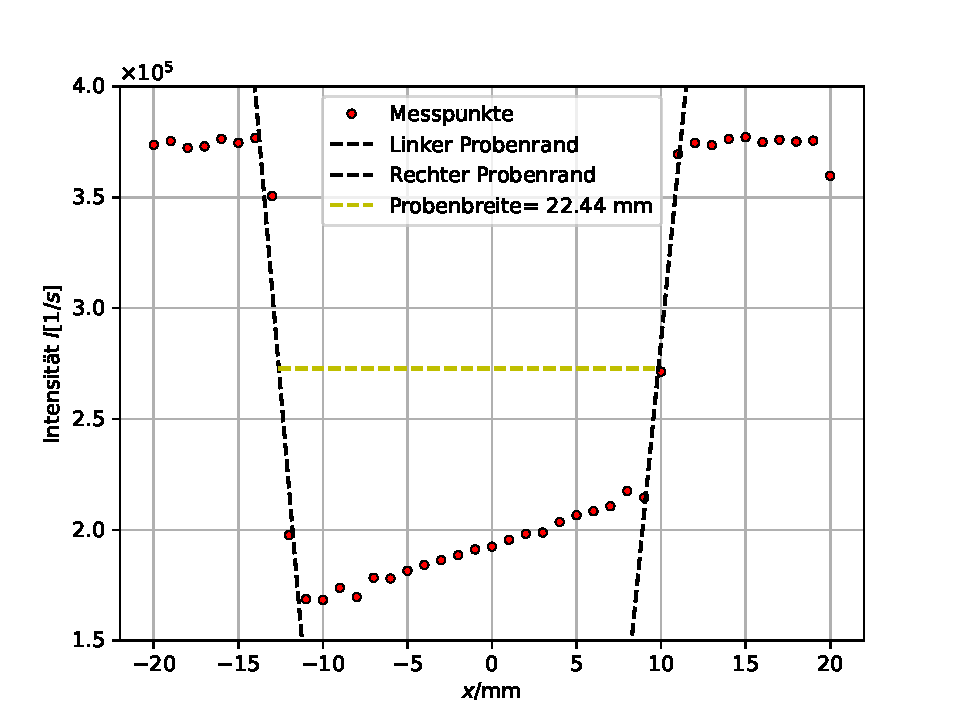
\includegraphics[width=0.8\textwidth]{plots/Xscan.pdf}
    \caption{X-Scan zur Bestimmung der Probenbreite}
    \label{fig:Xscan}
\end{figure}
Aus dem Rockingscan in Abbildung \ref{fig:Rocking} kann der Geometriewinkel bestimmt werden. Der Geometriewinkel ist der Winkel, bei dem die volle Intensität des Strahlers auf die Probe trifft.
Bei kleineren Winkeln ist die effektive Fläche, die der Strahl trifft, größer als die Probe selber, weshalb die Reflektivität dort natürlicherweise kleiner ist.
Der Rockingscan misst nun die Intensität bei Drehung der Probe im Strahl. Die Winkel bei denen die Intensität jeweils auf 0 abfällt markiert dabei jeweils den Geometriewinkel. 
Durch Mittelung ergibt sich der Geometriewinkel dann zu 
\begin{equation*}
    \theta_{\text{G}} = \SI{0.54(0)}{\degree}.
\end{equation*}
Alternativ lässt dich der Geometriewinkel auch durch Gleichung \eqref{eq:geometriewinkel} aus der gemessenen Strahlbreite und Probenbreite bestimmen. 
Damit ergibt sich der Geometriewinkel zu $\theta_{\text{G}} = \SI{0.41}{\degree}$. Wenn statt der gemessenen Probenbreite die theoretische Breite von $d_0=\SI{20}{\milli\meter}$ eingesetzt wird, ergibt sich $\theta_{\text{G}} = \SI{0.46}{\degree}$.
Für die Korrektur der Reflektivitätsmessung ist im Folgenden der Messwert des Rockingscans verwendet worden.
\begin{figure}[H]
    \centering
    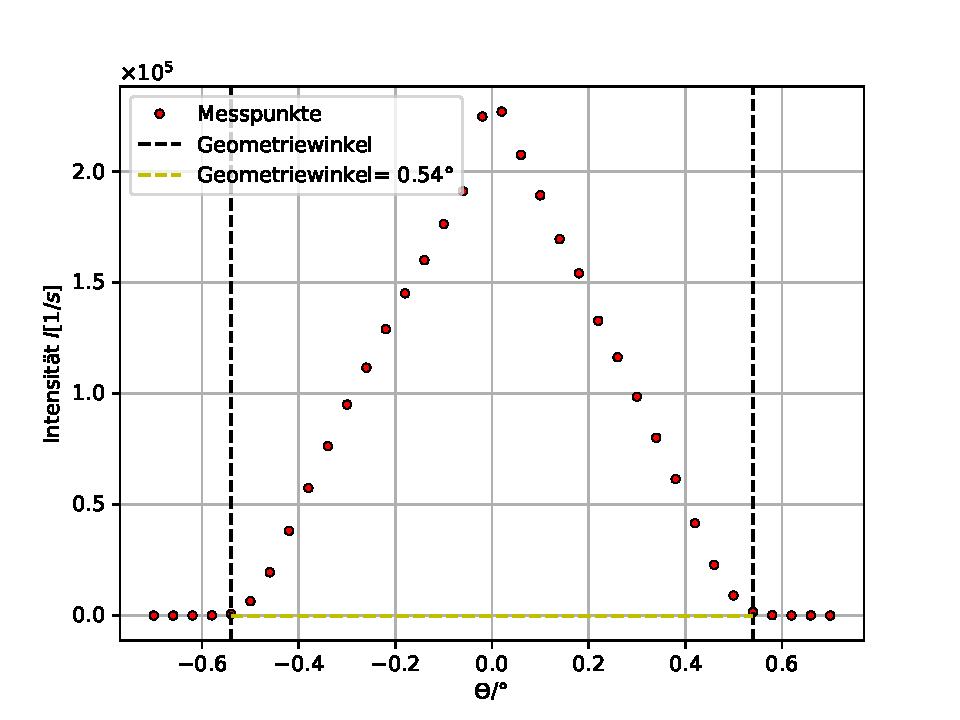
\includegraphics[width=0.8\textwidth]{plots/Rocking.pdf}
    \caption{Rockingscan zur Bestimmung des Geometriewinkels}
    \label{fig:Rocking}
\end{figure}
\subsection{Bestimmung der Rauigkeit und des Brechungsindex von Grenzschichten}
In Abbildung \ref{fig:Reflektionsmessung} ist die Messung des Reflexionsgrads in Abhängigkeit des Einfallswinkels dargestellt.
Zusätzlich ist eine Messung verschoben vom Beugungsmaximum aufgenommen worden, um die Diffuse Streuung zu messen. Durch Abzug der Messwerte 
der diffusen Streuung kann die wahre Reflektivität der Probe bei bestimmten Winkeln bestimmt werden. Dies ist ebenfalls in Abbildung \ref{fig:Reflektionsmessung} dargestellt.
Die Diffuse Messung ist ebenfalls eingezeichnet. Zu besseren Übersichtlichkeit sind Messpunkte mit einer Intensität von 0 nicht eingezeichnet worden.
\begin{figure}[H]
    \centering
    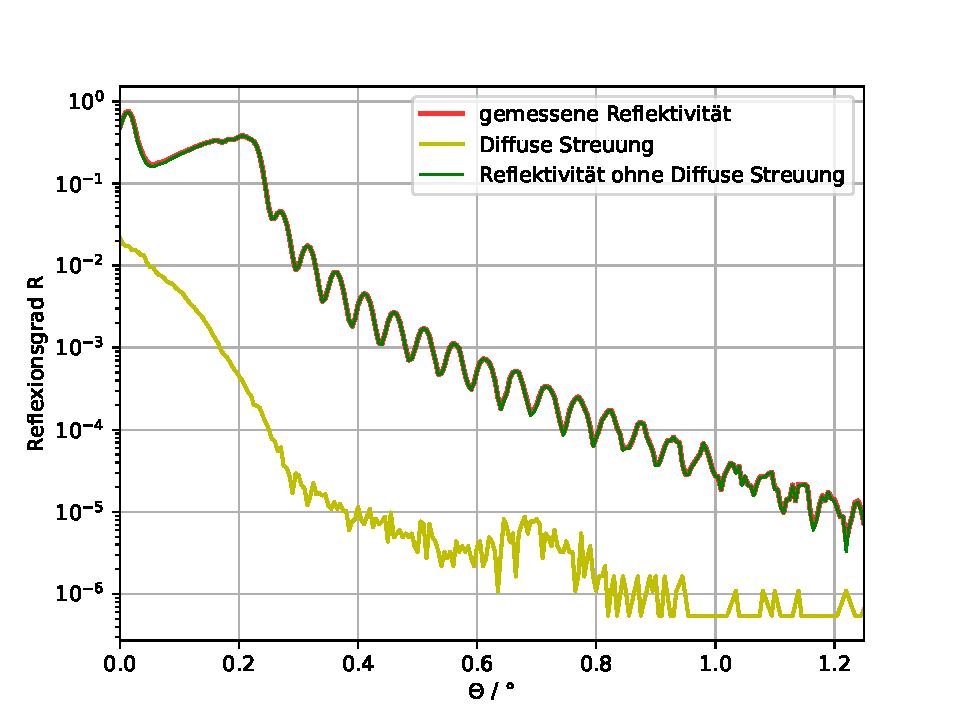
\includegraphics[width=0.8\textwidth]{plots/Reflektionsmessung.pdf}
    \caption{Reflexionsmessung in Abhängigkeit des Einfallswinkels}
    \label{fig:Reflektionsmessung}
\end{figure}
Nun soll die Messung noch um den Geometriefaktor aus Gleichung \eqref{eq:geometriefaktor} korrigiert werden. Dies ist in Abbildung \ref{fig:KorrigierteReflektionsmessung} dargestellt.
Diese Kurve kann mit der theoretischen Fresnelreflektivität verglichen werden. Dabei wird angenommen, dass die Probe ein unendlich ausgedehnter Siliziumkristall mit 
einer Diffusion von $\delta=7.6$ \cite{m-tolan2013} ist. Damit kann über Gleichung \eqref{eq:alpha} und \eqref{eq:Fresnel} die ideale Frenelreflektivitätskurve bestimmt werden und eingezeichnet werden.
Da bekannt ist, dass die Probe nicht aus zwei Schichten mit unterschiedlicher Dispersion $\delta$ besteht, können die Oszillationen, welche von den 
Fresnelkoeffizienten nicht vorhergesehen werden, als Kiessig-Oszillationen identifiziert werden. Aus Gleichung \eqref{eq:dicke} kann die Schichtdicke $d$ aus den Abständen der Minima und der Wellenlänge 
der $K_{\alpha}$-Linie von Kupfer $\lambda=\SI{1.54}{\angstrom}$ bestimmt werden.\cite{m-tolan2013}
Die Minima wurde über die Scipy-Funktion Findpeaks gefunden. Die Differenzen der Minima sind gemittelt worden zu $\Delta \theta = \SI{0.049(0.004)}{\degree}$.
Damit ergibt sich die Schichtdicke zu 
\begin{equation*}
    d = \SI{89(8)}{\nano\meter}.
\end{equation*}
\begin{figure}[H]
    \centering
    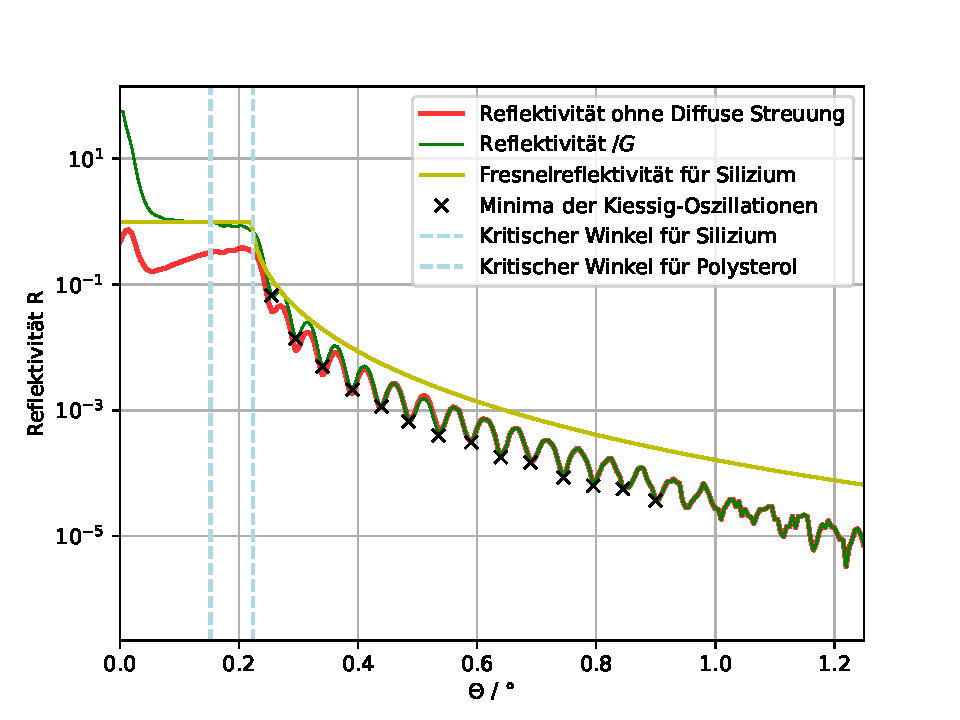
\includegraphics[width=0.8\textwidth]{plots/KorrigierteReflektionsmessung.pdf}
    \caption{Geometriefaktorkorrektur der Reflexionsmessung und Messung der Minima der Kiessig-Oszillationen}
    \label{fig:KorrigierteReflektionsmessung}
\end{figure}
Eine weitere Möglichkeit Informationen über Probe zu erhalten ist durch die Anwendung des Paratt-Algorhitmus. Dabei können 7 Parameter von außen vorgegeben werden. 
Die Dispersion $\delta$, die Absorptionskoeffizienten $\beta$ die Rauigkeit $\sigma$ der beiden Grenzflächen, sowie die Dicke $d$ der oberen Schicht.
Diese Parameter können so variiert werden, dass die Reflektivität der Probe möglichst gut angenähert wird. Das Ergebnis dieser Variation ist ist in Abbildung 
\ref{fig:Parattplot} dargestellt. Die Parameter betragen
\begin{align*}
    \delta_{\text{Si}} &= \SI{7.1e-6}{} \\
    \delta_{\text{Pol}} &= \SI{3.5e-6}{} \\
    \sigma_{\text{Si}} &= \SI{11e-10}{\meter} \\
    \sigma_{\text{Pol}} &= \SI{15e-10}{\meter} \\
    \beta_1 &= \SI{6e-7}{} \\
    \beta_2 &= \SI{1e-8}{} \\
    d &= \SI{8.1e-8}{\meter}.
\end{align*}
Eine Variation der Schichtdicke $d$ variiert die Wellenlänge der Kiessing Oszillationen. Die Variation der Dispersion $\delta$ variiert den kritischen Winkel
und damit wo die Reflektivität abfällt. Damit lässt sich die Kurve als ganzes gut verschieben. Die Absorption $\beta$ variiert die Höhe der Oszillationen und auch etwas den Abfall der Reflektivität bei 
zunehmenden Winkel. Die Rauigkeit $\sigma$ variiert wie die Kurve geformt ist und wie sich die Höhe der Intensitätsmaxima logaritmisch verändern.
Bei gleicher Rauigkeit beider Schichten haben die Maxima mit wachsendem Winkel das gleiche Verhältnis zu ihren Minima. Bei wachsender Rauigkeit fällt 
die Reflektivität zunehmend exponentiell ab. Also in einem logarithmischen Plot nahezu linear. Bei keiner Rauigkeit geht die Kurve der Maxima mit der idelalen Fresnelreflektivität.
\begin{figure}[H]
    \centering
    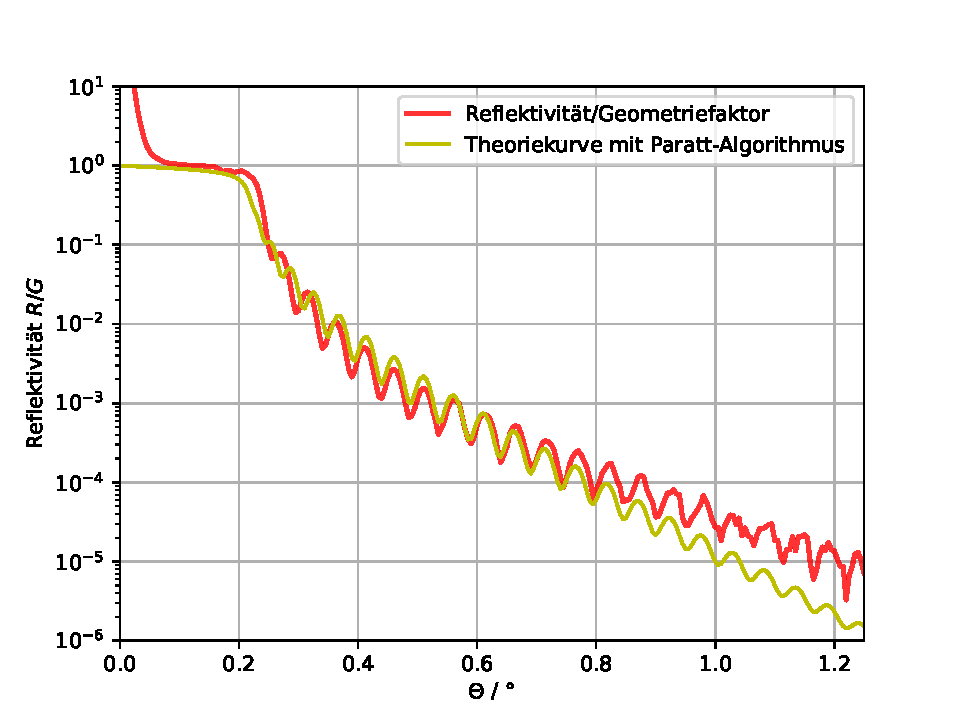
\includegraphics[width=0.8\textwidth]{plots/Parattplot.pdf}
    \caption{Näherung der Fresnelreflektivität durch das Paratt-Modell}
    \label{fig:Parattplot}
\end{figure}



